\documentclass[a4paper, 11pt]{article}
\usepackage{multirow}
\usepackage[spanish]{babel}
\usepackage{amsmath}
\usepackage{titling}
\usepackage{caption}
\usepackage{titlesec}
\usepackage{graphicx}
\usepackage[colorinlistoftodos]{todonotes}
\usepackage{wrapfig}
\usepackage[utf8]{inputenc}
\setcounter{secnumdepth}{4}

\makeatletter
\renewcommand\paragraph{\@startsection{paragraph}{4}{\z@}%
            {-2.5ex\@plus -1ex \@minus -.25ex}%
            {1.25ex \@plus .25ex}%
            {\normalfont\normalsize\bfseries}}
\makeatother
\setcounter{secnumdepth}{4} % how many sectioning levels to assign numbers to
\setcounter{tocdepth}{4}    % how many sectioning levels to show in ToC


\titleformat{\paragraph}
{\normalfont\normalsize\bfseries}{\theparagraph}{1em}{}
\titlespacing*{\paragraph}
{0pt}{3.25ex plus 1ex minus .2ex}{1.5ex plus .2ex}
\begin{document}
\renewcommand{\contentsname}{Lista de Contenidos}
\renewcommand{\listfigurename}{Lista de Figuras}
\renewcommand{\listtablename}{Lista de Tablas}
\renewcommand{\tablename}{Tabla}
\tableofcontents
\listoffigures
\listoftables
\thispagestyle{empty}
\newpage
\newcommand{\angstrom}{\mbox{\normalfont\AA}}

\begin{abstract}
En el siguiente experimento se determina de que material es una muestra a partir de las gráficas de esfuerzo-deformación y su dureza, para realizar esto primero se nos fue otorgada una muestra polimérica, del cual se obtuvo una probeta para posteriormente medir su dureza, luego se hizo el ensayo de tracción, para este tipo de materiales se realiza varias veces el mismo ensayo ya que existen diversas perturbaciones que influyen en el material, y de esta forma se obtiene un promedio que caracteriza de mejor manera al material que al realizarlo sólo una vez, se procedió de forma similar  con respecto a la medición de la dureza en escala Shore A, al comparar las figuras de esfuerzo deformación y principales propiedades en manuales se obtuvo que los materiales fueron polietileno de baja densidad, material A, polietileno elastométrico altamente ramificado, material B y polietileno con baja ramificación para el material C.
\end{abstract}

\section{Teor\'ia}
\setcounter{page}{1}
Aunque probablemente muchas personas no lo han notado, los polímeros se encuentran en todos lados en plásticos, resinas, adhesivos, cintas adhesivas y su estructura común se caracteriza por la presencia de largas cadenas covalentes de átomos. Es una clase de materiales extraordinaria y versátil, con una enorme diferencia de valores para una propiedad, inclusive para el mismo polímero pero en diferentes estados físicos, por ejemplo el modulo de Young para un caucho típico puede ser tan bajo como 10 Mpa, mientras que una fibra de cristal líquido puede ser tan alta como 350 GPa, aproximadamente 35000 veces más alto. Otra propiedad aún más diferenciable es la conductividad eléctrica, los mejores aislantes pueden tener una conductividad tan baja como $10^{-18} \omega^{-1} m^{-1}$, mientras que una muestra de poli-acetileno dopado puede alcanzar una conductividad de $10^{4} \omega^{-1} m^{-1}$, aproximadamente $10^{22}$ veces más mayor.   
\\
\\
Los polímeros como se define de manera etimológica es un compuesto formado por varias(poli) partes(meros), esas partes son denominadas meros, el cual es la unidad básica de forma análoga a la celda cristalográfica en metales, estos meros se repiten y forman un polímero, por ejemplo la molécula de estireno es un monomero que contiene un enlace doble, los químicos han ideado métodos para enlazar moléculas de estireno, estireno por sí mismo es denominado monomero, pero al estar enlazado con cientos se lo denomina poliestireno como se muestra en la figura \ref{estireno}.\\

\begin{wrapfigure}[4]{l}[-2pt]{0.5\textwidth} 
\vspace{-1.2cm}
  \begin{center}
    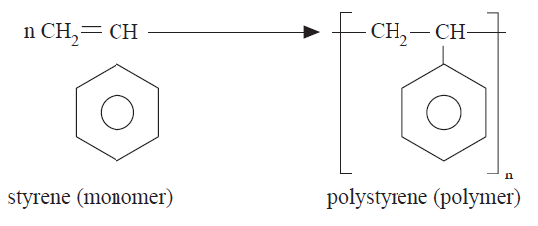
\includegraphics[scale=0.4]{estireno.png}
	\vspace{-0.5cm}    
     \caption{Estireno y Poliestireno}
    \label{estireno}
  \end{center}
\end{wrapfigure} 
\noindent
La unidad entre paréntesis es la unidad que se repite, a pesar que no son iguales, puesto que el estireno tiene un enlace doble y la unidad que se repite no, ambos poseen átomos idénticos ocupando posiciones relativas similares, la conversión de un monomero en polímero involucra un re-ordenamiento de los electrones.
\subsection{Clasificación de los polímeros}
Existen diversas formas para clasificar a los polímeros, las más útiles son las siguientes;\\

\subsubsection{Por su naturaleza} Los polímeros pueden ser naturales o sintéticos. Todos los procesos que ocurren en nuestro cuerpo (generación de energía a partir de los alimentos) es debido a la presencia de enzimas. Es posible que ocurra un deceso de la vida en caso de tener lugar a la deficiencia de estas enzimas, todas estas son polímeros de origen biológico. Su estructura, el cuál normalmente es muy compleja, no fue comprendida hasta la actualidad, por otro lado los polímeros sinteticos tienen estructuras más sencillas entre estos tenemos las fibras, elastómetros, plasticos, adhesivos, entre otros.\\

\subsubsection{Por su estructura} Lineal, ramificadas y en red, como se muestra en la figura \ref{lineal}, debe notarse que las estructuras son tridimensionales.\\
\begin{figure}[h!] 
\centering
\captionsetup{justification=centering}
    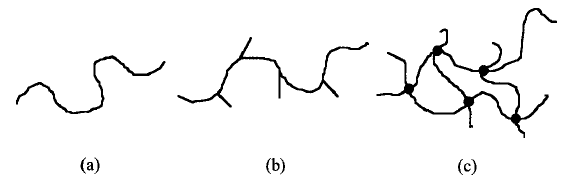
\includegraphics[scale=0.85]{clasestructura.png}
     \caption{Polímeros según su estructura; a) Lineal, b) Ramificadas y c) En red}
    \label{lineal}
\end{figure}
    
\subsubsection{Por sus propiedades} 
Termoplásticos, termoestables y elastómetros.\\

Ya que las propiedades y la estructura se encuentran relacionadas, será expuesta una breve descripción acerca de los tipos de polímeros con respecto a su clasificación.
\paragraph{Termo-plásticos} Forma la mayoría de los polímeros en uso, consisten en moléculas lineales o ramificadas, son suaves y se derriten con el calentamiento, por lo tanto pueden ser moldeadas y re-moldeadas al calentarlas, en el estado fundido consiste en una masa sin orden de moléculas. Al enfriarse puede transforma en vidrio (un tipo de líquido congelado), por debajo de la temperatura denominada temperatura de transición vítrea,o se cristaliza. En caso de cristalizarse y se hace de forma parcial, el resto que queda en forma líquida se la denomina amorfa, pero de preferencia se la denomina forma no cristalina.

\paragraph{Caucho} Son redes de polímeros ligeramente reticulados,  y es posible extenderlos de forma reversible una basta deformación. Cuando no se encuentra estirado este tiene moléculas arbitrariamente enredadas que son estiradas junto con el material, esto causa que las cadenas se ordenen, y por lo tanto el material tiene menos entropía, y la fuerza reconstructiva se debe a su menor entropía, puesto que la entropía siempre aumenta en todo proceso. Las retículas evitan que las moléculas se solapen unas a otras cuando el material es estirado. En enfriamiento, los cauchos se cristalizan parcialmente, al calentarse no se derriten de una forma convencional, no existe fluencia del material debido a las retículas.

\paragraph{Termo-estables} Son redes de polímeros altamente retículados el cual es lo que define la densidad de la red de tres dimensiones, normalmente son rígidos, no se pueden fundir al ser calentados y se descomponen cuando la temperatura es lo suficientemente alta, su nombre surge ya que es necesario primero calentar los polímeros de este tipo para dar lugar a la forma reticular , como ejemplo se tiene; resinas epoxicas, fenol y urea-formaldeida.

\subsubsection{Polímeros de cristal líquido (LCPs)} 
Es un subconjunto de los termoplásticos, consideremos primero cristales líquidos no poliméricos. Los tipos más simples son moléculoas en forma de barra, tipicamente como en la figura \ref{lcp}.

\begin{figure}[h!] 
\centering
    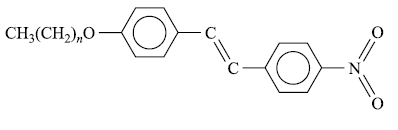
\includegraphics[scale=0.9]{lcp.png}
     \caption{Polímero de Cristal Líquido}
    \label{lcp}
\end{figure}
\
\\
En un rango de temperaturas las moléculas tienden a alinearse de forma paralela una a otra, pero no se incluye en cristales, esto da lugar a la formación de regiones anisotrópicas, el cuál le da propiedades ópticas que son ampliamente usadas para pantallas. 
Este tipo de polímeros esta clasificado en dos grupos principales:

\noindent
\paragraph{LCPs de Cadena principal} 
Son materiales rígidos que soportan altas temperaturas y usualmente se usan de tal forma que tenga una alta orientación molecular, las cadenas se encuentran alineadas y paralelas una a otra como se muestra en la figura \ref{cadenas_lcp}(a).

\paragraph{LCPs de Cadena Lateral} Puede ser usado como un material óptico no lineal, su ventaja es que es posible incorporarlo en un polímero, ya que  se encuentra enlazado químicamente por cadenas laterales, algunos grupos tienen propiedades ópticas útiles pero no se disuelven en un polímero, su representación esquemática es similar a la que se muestra en la figura \ref{cadenas_lcp}(b).\\
\begin{figure}[h!] 
\centering
\captionsetup{justification=centering}
    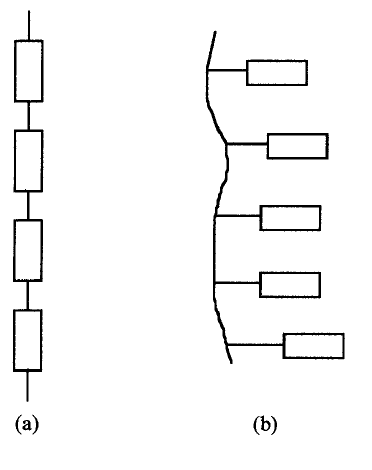
\includegraphics[scale=0.75]{cadenas_lcp.png} 
     \caption{Representación esquemática de las cadenas de un polímero LCPs a)Cadena Principal y b)Cadena Lateral}
    \label{cadenas_lcp}
\end{figure}
\subsection{Polimerización}
 Las reacciones para una polimerización en cadena de monómeros como el etileno para la formación de polímeros lineales como el polietileno puede dividirse en las siguientes etapas: iniciación, propagación y terminación.
 \subsubsection{Iniciación}
 Para la polimerización en cadena del etileno puede utilizarse uno de los distintos tipos de catalizadores. En esta discusión consideraremos el uso de peróxidos orgánicos los cuales actúan como generadores de radicales libres. Un radical libre puede definirse como un grupo de átomos que tienen un electrón libre y que puede enlazarse de forma covalente con un electron libre de otra molécula. Consideremos primero cómo una molécula de peróxido de hidrógeno. $H_{2}O_{2}$, puede descomponerse en dos radicales libres $2(H-O)$, con un electrón libre del átomo de oxígeno. En la polimerización en cadena del etileno por radicales libres un peróxido orgánico puede descomponerse de la misma forma que hemos visto para el peróxido de hidrógeno. Si $R-O-O-R$ representa un peróxido orgánico, donde R es el grupo químico, entonces por calentamiento, este peróxido puede descomponerse en dos radicales libres de una forma similar al peróxido de hidrógeno conforme hemos visto anteriormente, $2(R-O)$, con el electrón libre en el átomo de oxígeno.\\
Uno de los radicales libres creados por la descomposición del peróxido orgánico puede reaccionar con una molécula de etileno para formar un nuevo radical libre. El radical libre de esta manera actúa como un catalizador iniciador de la polimerización del etileno.
\subsubsection{Propagación}
El proceso de aumentar la cadena del polímero por sucesivas adiciones de unidades de monómero se denomina propagación. El doble enlace al final de la unidad de monómero de etileno puede ser abierto, generar un radical libre y enlazarse de forma covalente. Así, la cadena polimérica se extiende, siendo el último carbono el átomo que posee en electrón libre.
\\

Las cadenas de polímero mantienen el crecimiento espontáneamente porque la energía del sistema químico disminuye por el proceso de polimerización en cadena. Esto es, la suma de las energías de los polímeros producidos es menor que la suma de las energías de los monomeros que producen los polímeros. Los grados de polimerización (GP) de los polímeros producidos por la polimerización en cadena varía con el material polimérico. También el GP promedio varía. 

\subsubsection{Terminación}
En la etapa de terminación puede concluir el crecimiento de la cadena por la adición de un radical libre de acabado o cuando dos cadenas en crecimiento se combinan. Otra posibilidad es que trazas de impurezas puedan terminar la cadena polimérica. Los termoplásticos consisten en cadenas de polímeros de muchas longitudes diferentes, cada una de las cuales tiene su propio peso molecular y grado de polimerización.

\subsection{Procesos utilizados para materiales termo-plásticos}
\subsubsection{Moldeo por Inyección}
Es uno de los métodos de procesado más importantes para dar forma a los materiales termoplásticos. La maquinaria moderna de moldeo por inyección utiliza un mecanismo de enroscado alternativo para fundir el plástico e inyectarlo en un molde Fig.\ref{maquina_moldeo}. Una maquinaria más anticuada de moldeo por inyección utiliza un percutor para la inyección del material fundido. Una de las principales ventajas del método de enroscado alternativo sobre el método percutor es que el enroscado alternativo reparte el material fundido más homogéneamente para la inyección. En el proceso de moldeo por inyección, se introducen los gránulos plásticos desde una tolva, a través de un orificio, al cilindro de inyección sobre la superficie de un tornillo rotativo que los lleva hacia el molde Fig.\ref{proceso_inyeccion}(a). La rotación del tornillo empuja los gránulos contra las paredes calientes del cilindro, produciendo su fusion debido al calor de compresión, fricción y al calor de las paredes del cilindro Fig.\ref{proceso_inyeccion}    (b). Cuando se fusiona suficiente material plástico en el molde final del tornillo, el tornillo para y por movimiento de percusión inyecta un disparo de material fusionado a traves de un orificio de colada y entonces lo introduce dentro de las cavidades cerradas del molde Fig.\ref{proceso_inyeccion}(c). El tornillo mantiene la presión del material plástico introducido en el molde durante un corto periodo de tiempo para permitir su solidificación y entonces se retrae. El molde se enfría con agua para rapidamente bajar de temperatura la pieza plástica. Finalmente se abre el molde y la pieza es expulsada del molde con aire o mediante eyectores de puntas empujados por muelles Fig.\ref{proceso_inyeccion}(d). Entonces se cierra el molde y comienza un nuevo ciclo. \\
\\
Las principales ventajas del moldeo por inyección son:
\begin{itemize}
\item[1] Pueden producirse piezas de gran calidad a alta velocidad de producción.
\item[2] El proceso tiene relativamente bajos costes de mano de obra.
\item[3] Pueden producirse buenos acabados superficiales de las piezas moldeadas.
\item[4] El proceso puede automatizarse ampliamente.
\item[5] Pueden producirse formas complicadas.
\end{itemize}

\begin{figure}[h!] 
\centering
\captionsetup{justification=centering}
    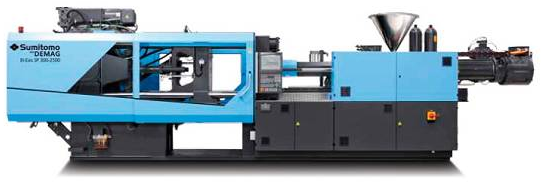
\includegraphics[scale=0.75]{maquina_moldeo.png} 
     \caption{Máquina de Moldeo por Inyección}
    \label{maquina_moldeo}
\end{figure}

Mientras que las principales desventajas del moldeo por inyección son:
\begin{itemize}
\item[1] Los altos costes de la maquinaria suponen la realización de una gran cantidad de piezas para la amortización de la máquina.
\item[2] El proceso debe ser estrechamente controlado para obtener un producto de calidad.
\end{itemize}
\begin{figure}[h!] 
\centering
\captionsetup{justification=centerlast}
    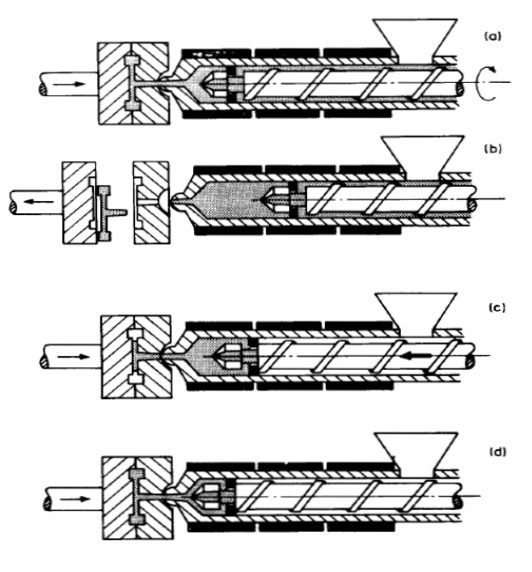
\includegraphics[scale=0.5]{proceso_inyeccion.png} 
     \caption{Secuencia de operaciones para el proceso de moldeo por inyección por tonillo rotativo de materiales plásticos, a)Se reparten los gránulos de plástico mediante un tambor en un tornillo giratorio. b) Se funden los gránulos de plástico mientras se desplazan a lo largo del tornillo giratorio y cuando hay suficiente material fundido al final del tornillo, el tornillo para de rotar. c) El tambor del tornillo se adelante con un movimiento de percusión e inyecta el plástico fundido a través de una abertura dentro de un sistema de canales y puertas dentro de la cavidad de un molde cerrado. d) El tambor del tornillo es retirado y la pieza y la pieza acabada de plástico expulsada.}
    \label{proceso_inyeccion}
\end{figure}
\subsubsection{Extrusión}
La extrusión es otro de los importantes métodos de procesado utilizados para los termoplásticos. Algunos de los productos manufacturados por el exceso de extrusión son tubos, varillas, láminas y todo tipo de formas. La máquina extrusora también se utiliza para realizar materiales compuestos plásticos para la producción de especies en bruto sin conformar, como bolitas, y para recuperación de residuos de materiales termoplásticos.\\
En el proceso de extrusión la resina de termoplástico se introduce en un cilindro caliente, mediante un tornillo rotatorio se fuerza al plástico fusionado a través de una abertura (o aberturas) en un molde adecuado para generar formas continuas Fig.\ref{maquina_extrusora}. Después de salir del moldeo la pieza debe enfriarse por debajo de su temperatura de transición para asegurar su estabilidad dimensional. El enfriamiento se realiza generalmente por chorro de aire mediante un sistema de refrigeración por agua.

\begin{figure}[h!] 
\centering
\captionsetup{justification=centering}
    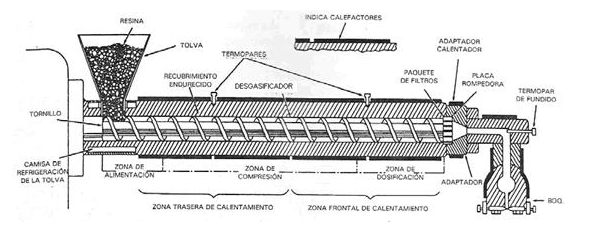
\includegraphics[scale=0.75]{maquina_extrusora.png} 
     \caption{Máquina Extrusora}
    \label{maquina_extrusora}
\end{figure}

\subsection{Normas ASTM}
Es necesario conocer algunas de las normas para realizar las mediciones según lo establecido por  ASTM(American Standards Test Methods) para definir la geometría de la probeta para determinar el esfuerzo de tensión de un material plástico como lo define la norma ASTM D 638-00~\cite{astmd638}, así como también es necesario conocer la norma ASTM D 256~\cite{astmd256} para determinar la resistencia de impacto de un material plástico, se debe considerar lo establecido en la norma ASTM D 2240-00~\cite{astmd2240} para medir la dureza de los diferentes tipos de plásticos.


\begin{figure}[h!] 
\centering
\captionsetup{justification=centering}
    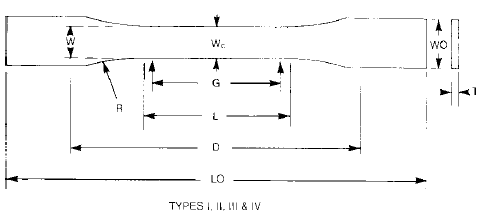
\includegraphics[scale=0.75]{probetas.png} 
     \caption{Geometría de la probeta}
    \label{probeta}
\end{figure}


\subsubsection{ASTM D 638-00}
Esta norma esta definida para determinar las propiedades de tracción de los plásticos, estableciendo previamente las condiciones de prueba como pre-calentamiento, temperatura, humedad, y velocidad de prueba de la máquina, este método puede ser usado para probetas de un espesor máximo de 14mm, los resultados obtenidos sirven para caracterizar al material de prueba.
Para obtener valores relevantes es necesario realizar el ensayo como mínimo cinco veces cuando el material es isotrópico en caso de ser anisotrópico se realiza cin ensayos en dirección normal y cinco en dirección transversal.
Para la geometría establecida para la probeta es necesario que tipo de plástico se tiene, es decir, si este es un plástico rígido o semirígido y con el espesor de la muestra se establece si el tipo es I, II, III, IV o V, las dimensiones se encuentran definidas en la figura \ref{probeta} y en la tabla \ref{tabla}

\begin{table}[h]
\centering
\captionsetup{justification=centering}
    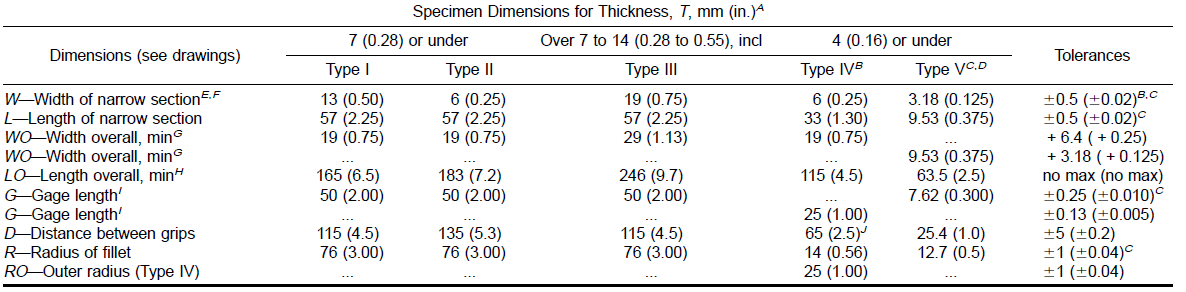
\includegraphics[scale=0.4]{tabla.png} 
     \caption{Medidas}
    \label{tabla}
\end{table}

\section{Procedimiento Experimental}

Se nos fue otorgada una muestra de un material polimérico desconocido, para preparar la muestra para posteriormente hacer el ensayo de tracción fue necesario primero usar la troqueladora Fig.\ref{troqueladora} (Marca: Ray-Ran, Modelo: RR/HCP, Código: EA-024, Serie: RR/HCP/147), se seleccionó una sección de la muestra del cual, sea posible luego hacer las diferentes mediciones de dureza, se obtuvo las diferentes mediciones de dureza Fig.\ref{dureza_shore} (Marca: Qualitest, Shore A, Identador: 0.5 in de diámetro y consta de un error sistemático) en la muestra polimérica como lo establece la norma ASTM D 2240-00, con un mínimo de cinco mediciones, y una distancia mínima de seis milímetros entre indentaciones, puesto que no se obtuvo la resistencia al impacto de la muestra no se usó la norma ASTM D 638-00.\\

Finalmente se realizó el ensayo de tracción con cinco diferentes probetas pero de igual dimensión como lo establece la norma ASTM D 256-00, ya que de esta forma es posible obtener resultados relevantes, puesto que existen diversos defectos o imperfecciones en el material y por lo tanto no es posible determinar valores con un sólo ensayo.

\section{An\'alisis de Resultados}

Al realizar el ensayo de tracción fue posible notar las variaciones en los resultados que ocurre, puesto a que la geometría de la probeta esta diseñada de tal forma que su ruptura sea en centro, pero en algunos casos eso no fue lo que ocurrió, esto se le atribuye a las imperfecciones que existen en la fabricación, de forma análoga que en los metales, las dislocaciones son los concentradores de esfuerzos y son las primeras secciones que fallan, de forma análoga sucede en los polímeros con las burbujas de aire que suelen tener cuando su elaboración es muy rápida y no da tiempo suficiente para que el aire interno salga, sino que el material encierra al aire formando pequeñas burbujas de aire en el interior.\\
\\
De acuerdo con los datos obtenidos en Sec.\ref{subsec:calculos} y comparando con los manuales a disposición ~\cite{no10} y ~\cite{no11}, se obtuvo que los materiales analizados fueron polietileno de baja densidad para el material A, ya que tiene un esfuerzo máximo bajo comparado con un polietileno de alta densidad, con respecto a la deformación máxima y al modulo de elasticidad se tiene resultados que estan dentro del intervalo del polietileno de alta densidad Fig.\ref{material_a}. En el material B la figura tiene un comportamiento que presentan los elastómetros de froma similar que lo hecho con el material A, se compara con datos de los manuales, en este caso es un polietileno elastométrico altamente ramificado, mientras mayor cantidad de ramificaciones tenga el material, será mayor la deformación que éste soportará como se observa en la Fig.\ref{material_b}, con respecto al material C se tiene una figura con un comportamiento muy similar al material B, pero difiere en la deformación máxima, en este caso es un polietileno con baja ramificación, por lo descrito anteriormente Fig.\ref{material_c}.


\section{Conclusiones}

Al concluir la práctica se logró corroborar de forma aproximada que material era cada uno de los que fueron sometidos a pruebas de tensión, siendo el material A polietileno de baja densidad, el material B un polietileno elastométrico altamente ramificado y el material C es menos ramificado que el material B.\\
La comparación de los materiales de acuerdo a la dureza no fue posible realizarla debido a que en cada caso se usó materiales diferentes, y sólo se obtuvo mediciones de dureza de un sòlo material que es diferente al usado en tracción, por tal motivo es imposible realizar una comparación aceptable.\\
Debido a la falta de información con respecto a las medidas de cada probeta no es posible determinar si la prueba de tensión fue realizada siguiendo lo establecido en la norma ASTM D-638-1, al desconocer completamente el material se procede a hacer probetas dependiendo de la dureza del material se define si es Tipo I,II,III o IV, y la norma establece hacer cinco probetas para cinco ensayos de tal forma que sea posible determinar una media y varianza de los valores, ya que se debe buscar que en cada ensayo la ruptura sea justo en el centro.\\
Ya que la empresa requiere que el material sea de alta resistencia mecánica, el cuál queda definido por el esfuerzo máximo y el modulo de elasticidad, es decir, mientras mayores sean estos valores, se considera que el material es más resistente, según los resultados obtenidos Sec.\ref{subsec:calculos} el que cumple con estas condiciones es el material B, el polietileno elastométrico altamente ramificado.  

\begin{thebibliography}{9}

\bibitem{polymer}
David I. Bower, An Introduction to Polymer Physics, (2002), Cambridge University Press,  United Kingdom, Cambidge.

\bibitem{no1}
Charles E. Carraher, Jr., Polymer Chemistry, Sixth Edition Revised and Expanded, (2003), Marcel Dekker, Inc., USA, New York.  

\bibitem{astmd2240}
American Society of the International Association for Testing and Materials, Standard Test Method for Rubber Property - Durometer Hardness, ASTM D 2240-00, Agosto 2000, Disponible en: http://www.abqindustrial.net/store/images/products/dmt/RX-DD/d2240.pdf, Fecha de Consulta: 19/08/2016 

\bibitem{astmd256}
American Society of the International Association for Testing and Materials, Standard Test Method for Determining the Izod Pendulum Impact Resistance of Plastics, ASTM D 256-02, Octubre 2002, Disponible en: http://www.mediafire.com/download/2yi0mdt2eg2a59u/ASTM\_D-256.pdf, Fecha de Consulta: 21/08/2016 

\bibitem{astmd638}
American Society of the International Association for Testing and Materials, Standard Test Method for Tensile Properties of Plastics, ASTM D 638-00, Febrero 2001, Disponible en: http://www.mediafire.com/download/6pry1zqreojpned/ASTM\_D-638.pdf, Fecha de Consulta: 21/08/2016 

\bibitem{no3}
Robert O. Ebewele, Polymer Science and Technology, (2000), CRC Press LLC, USA, New York

\bibitem{no4}
Escuela Superior Politécnica del Litoral, Facultad de Ingeniería Mecánica y Ciencias de la Producción, Área de Materiales, Laboratorio de Materiales de Ingeniería, Guía de la Práctica 5 "Polímeros", Agosto 2016, Guayaquil, Ecuador.

\bibitem{no5}
William D. Callister, Jr., Fundamentals of Materials cience and Engineering, Fifth Edition, John Wiley and Sons, Inc., (2002), New York, USA.  

\bibitem{no6}
William D. Callister, Jr., Fundamentals of Materials cience and Engineering, Fifth Edition, John Wiley and Sons, Inc., (2002), New York, USA, Ch. 13

\bibitem{no7}
Donald R. Askeland, Ciencia e Ingeniería de los Materiales, Tercera Edición, International Thomson Editors, (1998), Buenos Aires, Argentina, Cap. 15

\bibitem{no8}
William F. Smith, Fundamentos d la Ciencia e Ingeniería de Materiales, Tercera Edición, McGrawHill,(1998), Madrid, España, Cap. 9.

\bibitem{no9}
University of Notre Dame, Material Science, Disponible en: https://www3.nd.edu/manufact/MPEM\_pdf\_files/Ch10.pdf , Fecha de Consulta: 23/08/2016

\bibitem{no10}
J. Brandrup, E. H. Immergut, E.A. Grulke, Polymer Hand-Book, Fourth Edition, John Wiley and Sons, Inc., (1999), New York, USA.

\bibitem{no11}
J.E. Mark, Polymer Data Hand-Book, Oxford University Press, Inc., (1999)



\end{thebibliography}
\newpage      

\section{Anexos}

\subsection{Cálculos relevantes}\label{subsec:calculos}

Para obtener el modulo de elasticidad se relaciona la variación del esfuerzo y la variación de la deformación, ya que no se obtuvo una tabla de datos, se hizo una aproximación gráfica midiendo la escala mínima y relacionando de forma proporcional al extender la abscisa del punto hasta al eje obteniendo los siguientes datos para cada material;\\
\\
Material A\\
$\sigma_{m\acute{a}x}=11.6 MPa$\\
$\epsilon_{Ruptura}=245\%$\\
$\epsilon_{P.C.} = 0.3\frac{0.4}{2.5}=0.048$\\
$\sigma_{P.C.}=7.8 Mpa$\\     
$E=\frac{\sigma_{P.C.}}{\epsilon_{P.C.}}=0.15 GPa$\\
\\
\\
Material B\\
$\sigma_{m\acute{a}x}=18.2 MPa$\\
$\epsilon_{Ruptura}=811\%$\\
$\epsilon_{P.C.} = 0.9\frac{0.1}{2}=0.045$\\
$\sigma_{P.C.}=10 Mpa$\\     
$E=\frac{\sigma_{P.C.}}{\epsilon_{P.C.}}=0.222 GPa$\\
\\
\\
Material C\\
$\sigma_{m\acute{a}x}=17 MPa$\\
$\epsilon_{Ruptura}=362\%$\\
$\epsilon_{P.C.} = 0.4\frac{0.5}{2.15}=0.093$\\
$\sigma_{P.C.}=13.2 Mpa$\\     
$E=\frac{\sigma_{P.C.}}{\epsilon_{P.C.}}=0.141 GPa$\\

\newpage


\subsection{Gráficas Obtenidos}

\begin{figure}[h!] 
\centering
\captionsetup{justification=centering}
    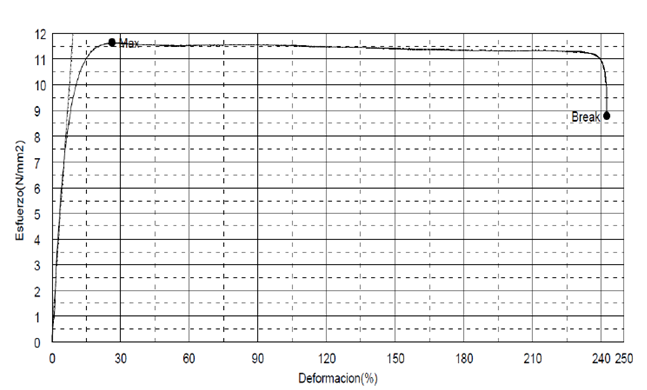
\includegraphics[scale=0.75]{material_a.png} 
     \caption{Material A}
    \label{material_a}
\end{figure}

\begin{figure}[h!] 
\centering
\captionsetup{justification=centering}
    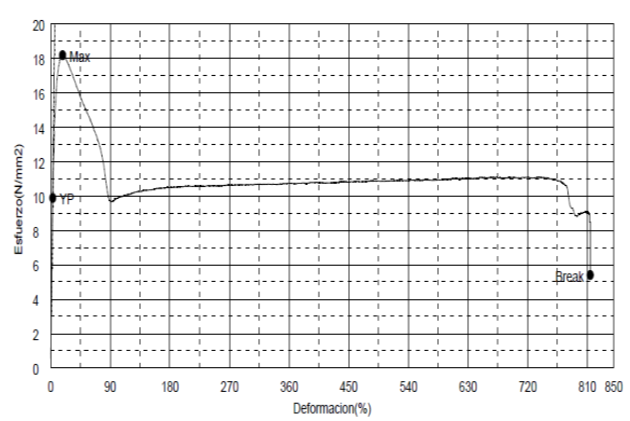
\includegraphics[scale=0.75]{material_b.png} 
     \caption{Material B}
    \label{material_b}
\end{figure}

\begin{figure}[h!] 
\centering
\captionsetup{justification=centering}
    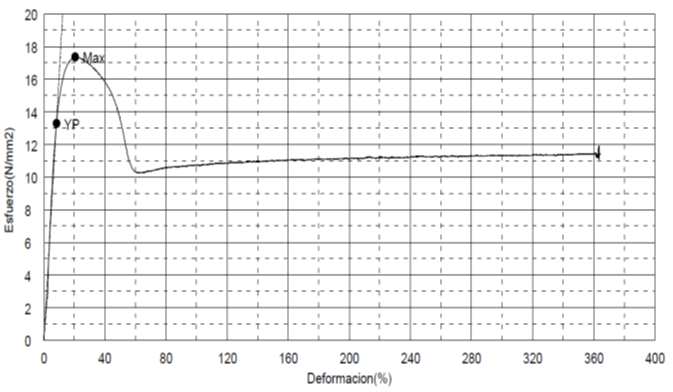
\includegraphics[scale=0.75]{material_c.png} 
     \caption{Material C}
    \label{material_c}
\end{figure}

\subsection{Equipos Usados}

\begin{figure}[h!] % indico que voy a poner una figura y [h] indica que la posición relativa, tambien puedo usar t = top entre otros.

\hfill
\begin{minipage}[t]{.45\textwidth}
\begin{center}
\captionsetup{justification=centering}
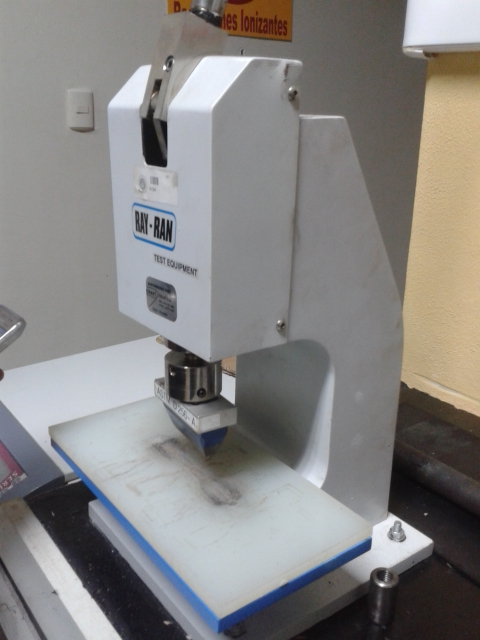
\includegraphics[scale=0.2]{troqueladora.png}
\caption{Troqueladora}
\label{troqueladora}
\end{center}
\end{minipage}
\hfill
\begin{minipage}[t]{.45\textwidth}
\begin{center}
\captionsetup{justification=centering}
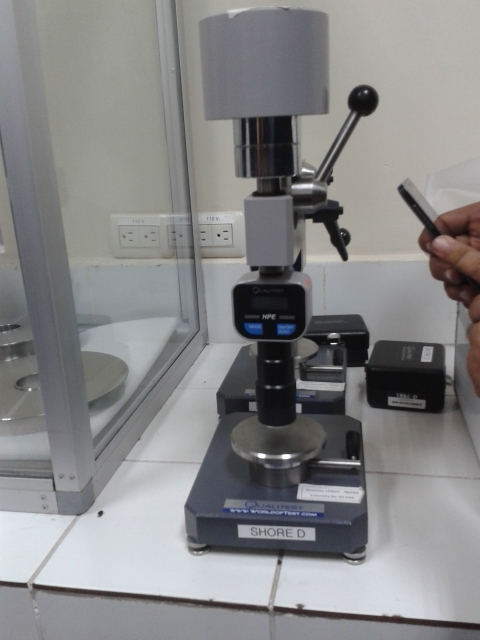
\includegraphics[scale=0.2]{dureza_shore.png}
\caption{Máquina para determinar dureza}
\label{dureza_shore}
\end{center}
\end{minipage}
\hfill
\end{figure}
\hfill
\newpage
\begin{figure}[h!] % indico que voy a poner una figura y [h] indica que la posición relativa, tambien puedo usar t = top entre otros.
\hfill
\begin{minipage}[t]{.45\textwidth}
\begin{center}
\captionsetup{justification=centering}
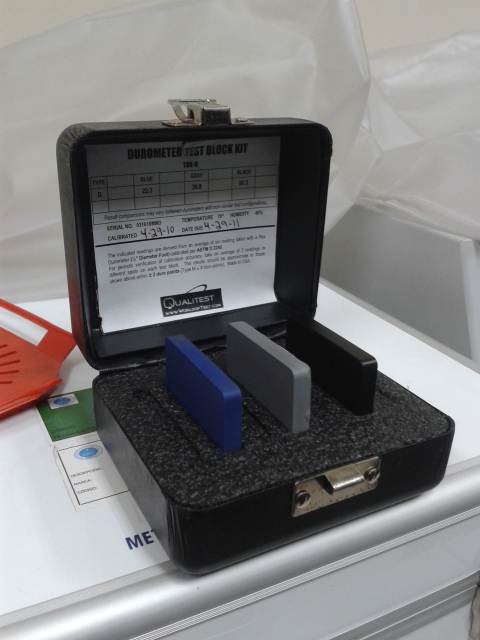
\includegraphics[scale=0.2]{patrones_dureza_shore.png}
\caption{Patrones para medir dureza}
\label{patrones_dureza_shore}
\end{center}
\end{minipage}
\hfill
\begin{minipage}[t]{.45\textwidth}
\begin{center}
\captionsetup{justification=centering}
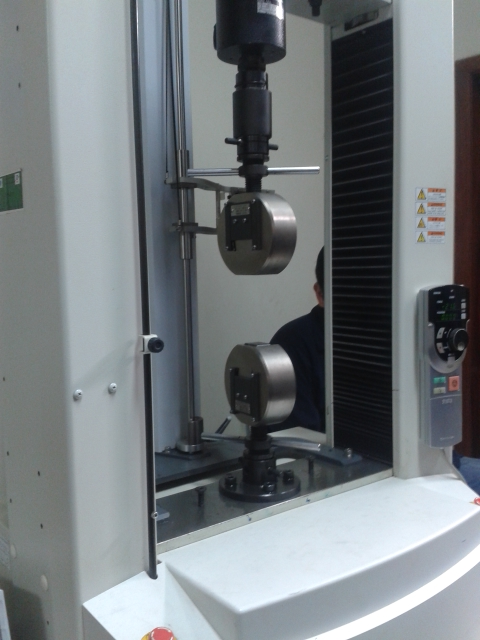
\includegraphics[scale=0.2]{maquina_universal_ensayos.png}
\caption{Máquina Universal de Ensayos}
\label{maquina_universal_ensayos}
\end{center}
\end{minipage}
\hfill
\end{figure}

\subsection{Mediciones de dureza}

\begin{table}[htbp]
\begin{center}
\begin{tabular}{|c|}
\hline
Shore A \\
\hline 
59.8 \\ \hline
62.0  \\ \hline
62.0 \\ \hline
62.9 \\ \hline
63.3 \\ \hline
62.4 \\ \hline
\end{tabular}
\caption{Dureza en material polimérico.}
\label{tabla:sencilla}
\end{center}
\end{table}
\section{Preguntas Evaluativas}
\subsection{¿Cuáles son las características y las propiedades físico-químicas de los polímeros que permiten diferenciarlos unos de otro?}
Entre las propiedades químicas que permiten diferenciar un polímero de otro es el grado de polarización que es la razón entre el peso molecular del polímero y el mero, la cantidad de ramificaciones que se encuentren en el polímero también es una de las propiedades relevantes para su caracterización, así como su dureza y las deformaciones y esfuerzos que son capaces de soportar.

\subsection{¿Qué significa ser resistente en material polimérico?}
Cuando se hace referencia a que un material polimérico es resistente, se debe a que este material soporta flexión, tensión y compresión. 

\subsection{¿Por qué hablamos de elongación en polímeros?}
La elongación es una de las propiedades principales que permite caracterizar a los polímeros, la elongación es un tipo de deformación y esta es simplemente el cambio en la forma que experimenta cualquier cosa bajo tensión. Cuando hablamos de tensión, la muestra se deforma por estiramiento, volviéndose más larga.

\subsection{¿Por qué hablamos de dureza en polímeros?}
La dureza es la resistencia a la indentación de un material, para los polímeros se usa la dureza Shore.

\subsection{¿En qué diferencia la dureza de la resistencia?}
La dureza y la resistencia se diferencian en que la dureza es la resistencia a la indentacion y la resistencia es la carga por unidad de area maxima que es capaz de soportar un material. 

\subsection{¿Qué indica que el polímero sea cristalino/no cristalino?}
Cuando un polímero es cristalino este tiene una resistencia mecánica mayor pero menor ductilidad, y menor deformación máxima a diferencia del no cristalino que por lo general es mas dúctil, se deforma mas que el cristalino, esto hace refencia a la estructura del material, siendo los cristalinos mas rígidos que los no cristalinos.

\subsection{¿Qué es temperatura de transición vítrea?}
Es la temperatura a la que el material disminuye su densidad, dureza y rigidez, y adicionalmente su elongación disminuye de una forma más notoria en comparación al resto de propiedades citadas.

\subsection{¿En qué se diferencia los polímeros termoplásticos y termoestables?}
Los materiales termoplásticos son aquellos que se pueden deformar y ser moldeados al aumentar la temepratura, a diferencia de los termoestables que al aumentar la temperatura no se funden ni se moldean si no que se descomponen.


\end{document}    